\chapter{EMTG Mission Types}
\label{chap:mission_types}

    \ac{EMTG} provides several transcription methods to model the flight of a spacecraft at various levels of accuracy. These methods are known in \ac{EMTG} as Mission Types. \ac{EMTG} provides Mission Types for chemical and low thrust spacecraft. Not all Mission Types are compatible with all of the propagation methods and perturbations discussed in Chapter \ref{chap:force_model_prop}. Table \ref{tab:mission_propagation_perturbation_compatibility} describes which perturbation and propagation methods can be used with each Mission Type. Setting perturbations for an incompatible Mission Type and propagation method in PyEMTG or the \ac{EMTG} options file will have no effect on the spacecraft force model and \ac{EMTG} will not notify the user that pertubations are not being applied.

    \begin{table}[H]
        \centering
        \begin{tabular}{lll}
        \hline
        Mission Type & Propagation & Perturbation Modeling \\ \hline
        \ac{MGAnDSMs} & Integrator or Kepler & Only with Integrator \\
        \ac{MGALT} & Kepler & Yes \\
        \ac{FBLT} & Integrator & Yes \\
        Coast Phase & Integrator or Kepler & Only with Integrator \\ 
        \ac{PSFB} & Integrator & Yes \\
        \ac{PSBI} & Kepler & Yes \\
        Probe Entry Phase & Integrator & Yes \\
        \hline
        \end{tabular}
        \caption{Mission Type, Propagation, and Perturbation Compatibility}
        \label{tab:mission_propagation_perturbation_compatibility}
    \end{table}


\section{Multiple Gravity Assist with n Deep Space Maneuvers (MGAnDSMs)}
\label{sec:MGAnDSMs}

    \acf{MGAnDSMs} transcription models the flight of a spacecraft using high-thrust chemical propulsion. This is done using two-point shooting to propagate a trajectory, where for a single phase the spacecraft is propagated forward in time from a left-hand boundary condition and backward in time from a right-hand boundary condition with a set of match point constraints to link the forward and backward half-phases together. The maneuvers are encoded as impulsive events, i.e. they happen instantaneously, and the optimizer may place maneuvers in any permitted location in the phase. The user chooses the maximum number of impulses a priori. If the specified number of impulses is more than what is needed, the optimizer will reduce the magnitude of any un-needed maneuvers to zero.     

    \noindent Selecting \ac{MGAnDSMs} for one or more Journeys activates the variable ``impulses per phase'' in the Journey Options tab which sets the maximum number of impulsive burns that can occur during the Journey. Spacecraft propagation can be modeled with Kepler or Integrator between instantaneous delta-v events at each DSM. Perturbations can only be applied with Integrator propagation by adding the perturbing forces to the central body gravitational force. 

    \noindent \ac{EMTG} will decrement the mass of the spacecraft according to the engine Isp specified in the Spacecraft Options section of PyEMTG (see Section \ref{sec:spacecraft_options}), the \ac{EMTG} Options file, or Spacecraft Configuration file (see Section \ref{sec:spacecraft_config}). This is labeled as ``Chemical Isp (s)'' in PyEMTG and as ``IspChem'' in the \ac{EMTG} Options file. In Figure \ref{fig:MGAnDSMs_mission_type}, $m_0$ refers to the mass of the spacecraft at the start of the Journey, $m_n$ to the mass after DSM $n$, and $m_f$ to the mass at the end of the Journey where $m_N = m_f$ after the final DSM in the Journey. The red arrows indicate the impulsive velocity change where $\mathbf{v}_n^-$ is the spacecraft velocity prior to the impulsive delta-v and $\mathbf{v}_n^+$ is the velocity after the impulsive delta-v.

    \begin{figure}[H]
        \centering
        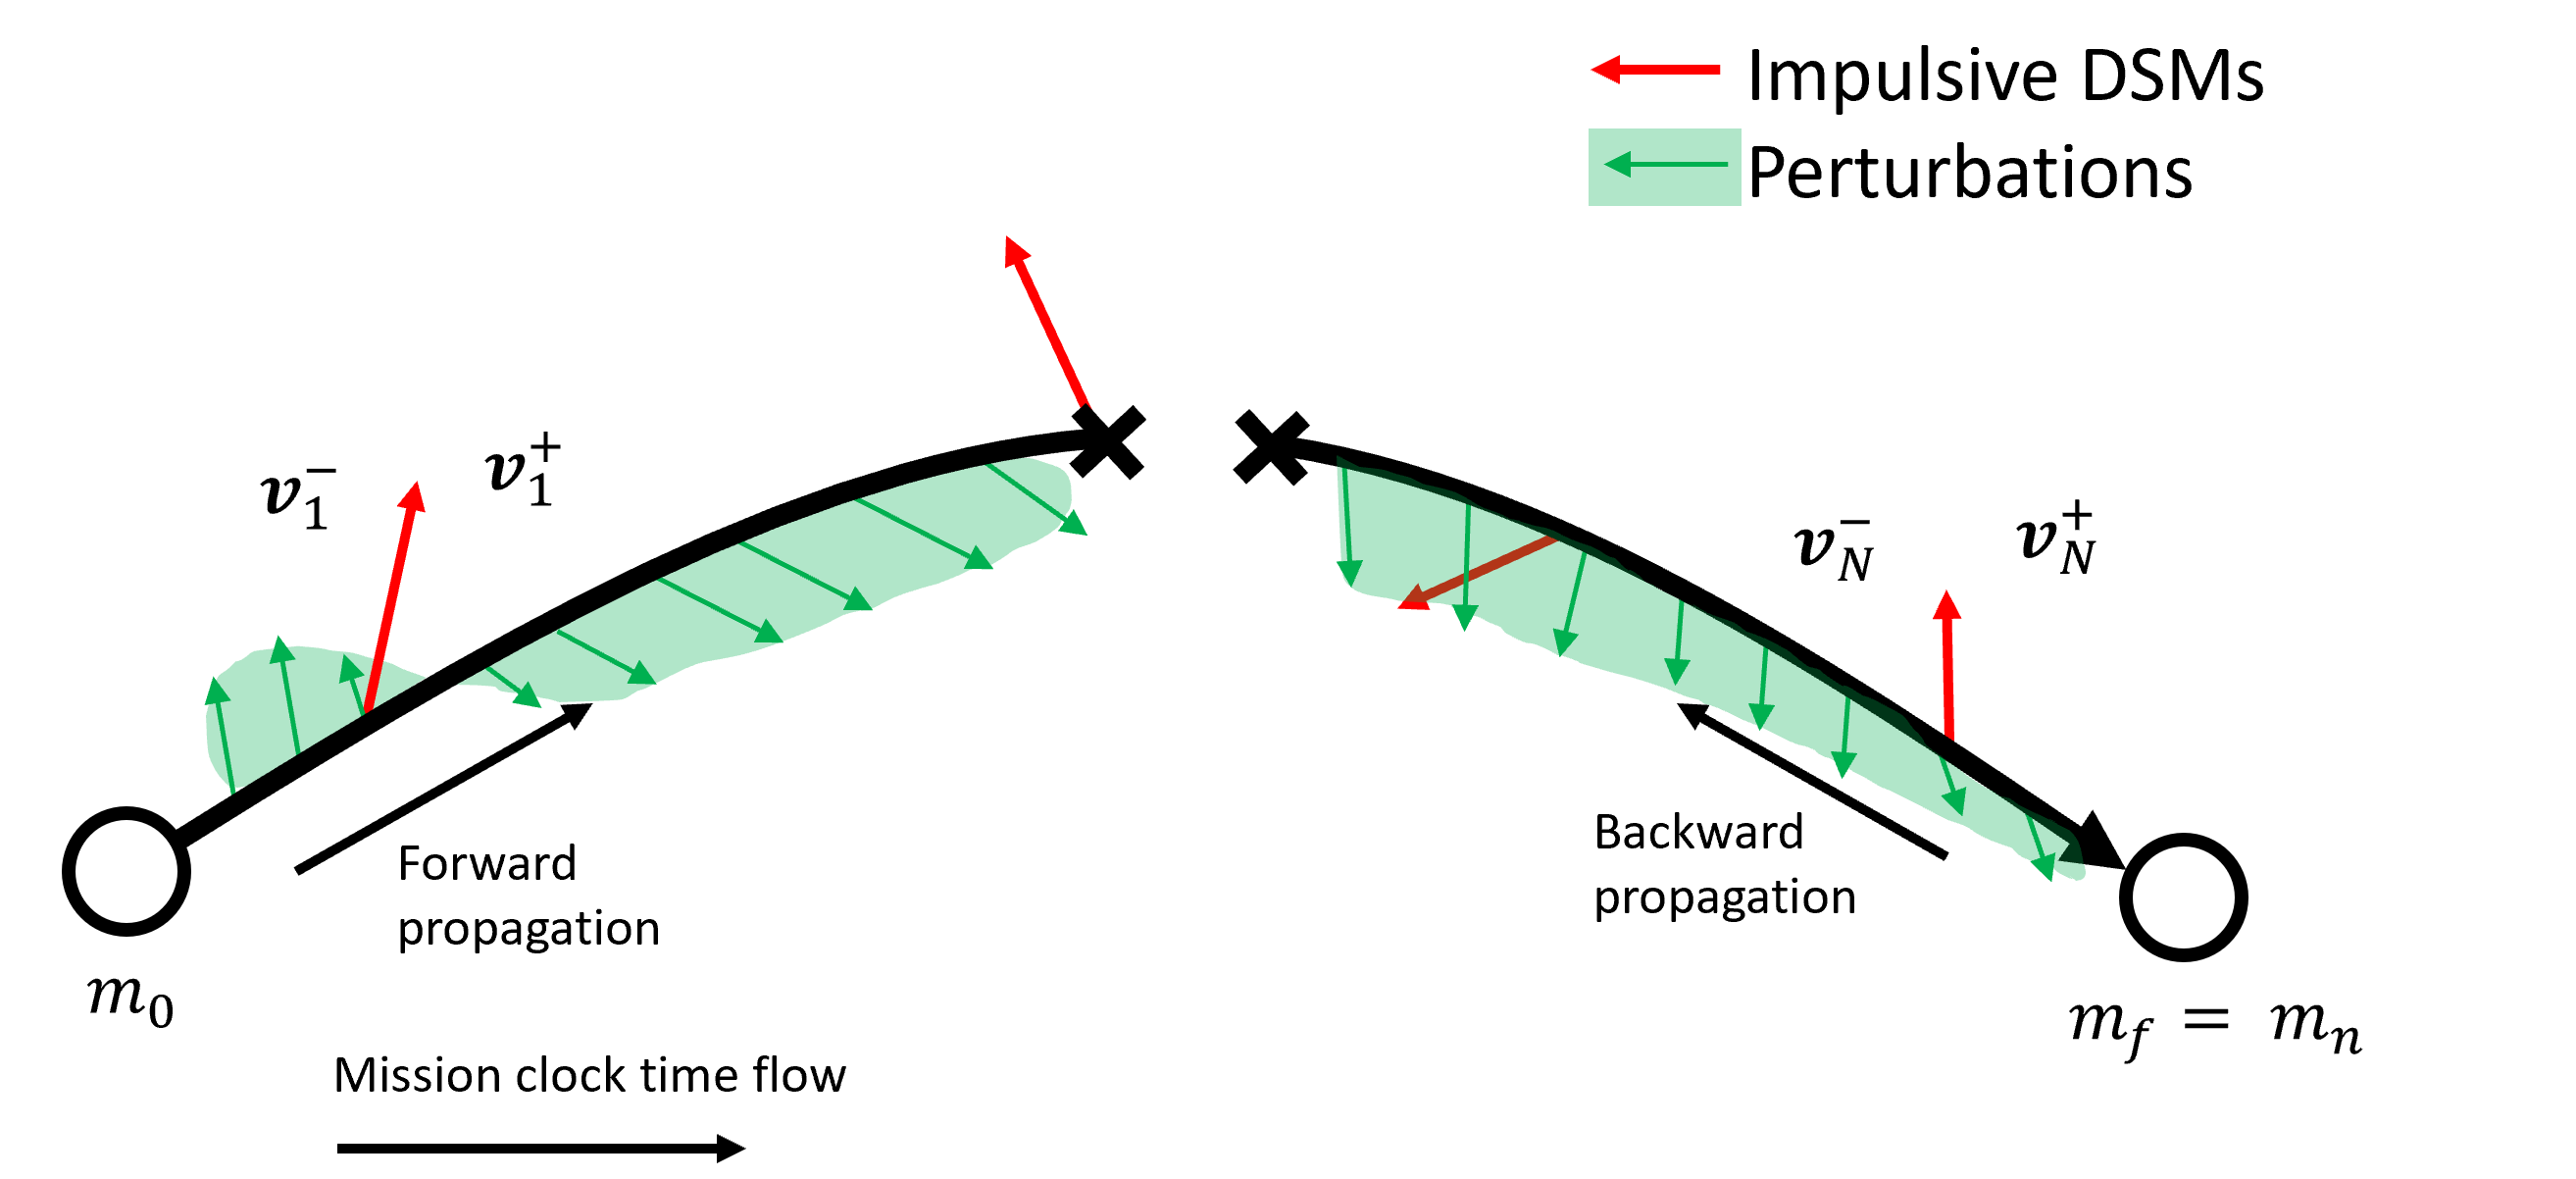
\includegraphics[width=0.9\textwidth]{../../shared_latex_inputs/images/mgandsms.png}
        \caption{\acf{MGAnDSMs}}
        \label{fig:MGAnDSMs_mission_type}
        %TODO update this figure to show mf = mN capital N like velocity
        % Where was this figure drawn? I only have a .png from docs/shared_latex_inputs
    \end{figure}

\section{Multiple Gravity Assist with Low-Thrust (MGALT)}
\label{sec:MGALT}

    \acf{MGALT} uses two-point shooting to propagate a trajectory. Each phase is propagated forward in time from a left-hand boundary condition and backward in time from a right-hand boundary condition with a set of match point constraints to link the forward and backward half-phases together. \ac{MGALT} then models each Journey using the Sims-Flanagan transcription and Kepler propagation. A bounded-impulse delta-v is applied at each segment to model the spacecraft's thrust; the magnitude of the impulse is limited to the maximum delta-v that could be achieved by thrusting constantly across the segment. If any perturbations are turned on, they are applied in a similar manner: the perturbing force(s) are evaluated at the point at which each propulsive delta-v is applied. The effect of the perturbing acceleration(s) across the segment is approximated by multiplying the acceleration by the time between segments. The perturbing ``delta-v'' is then added to the propulsive delta-v to get the full impulse applied to the spacecraft. As a result, \ac{MGALT} can approximate the effect of perturbing accelerations without using integrator propagation. 

    \begin{figure}[H]
        \centering
        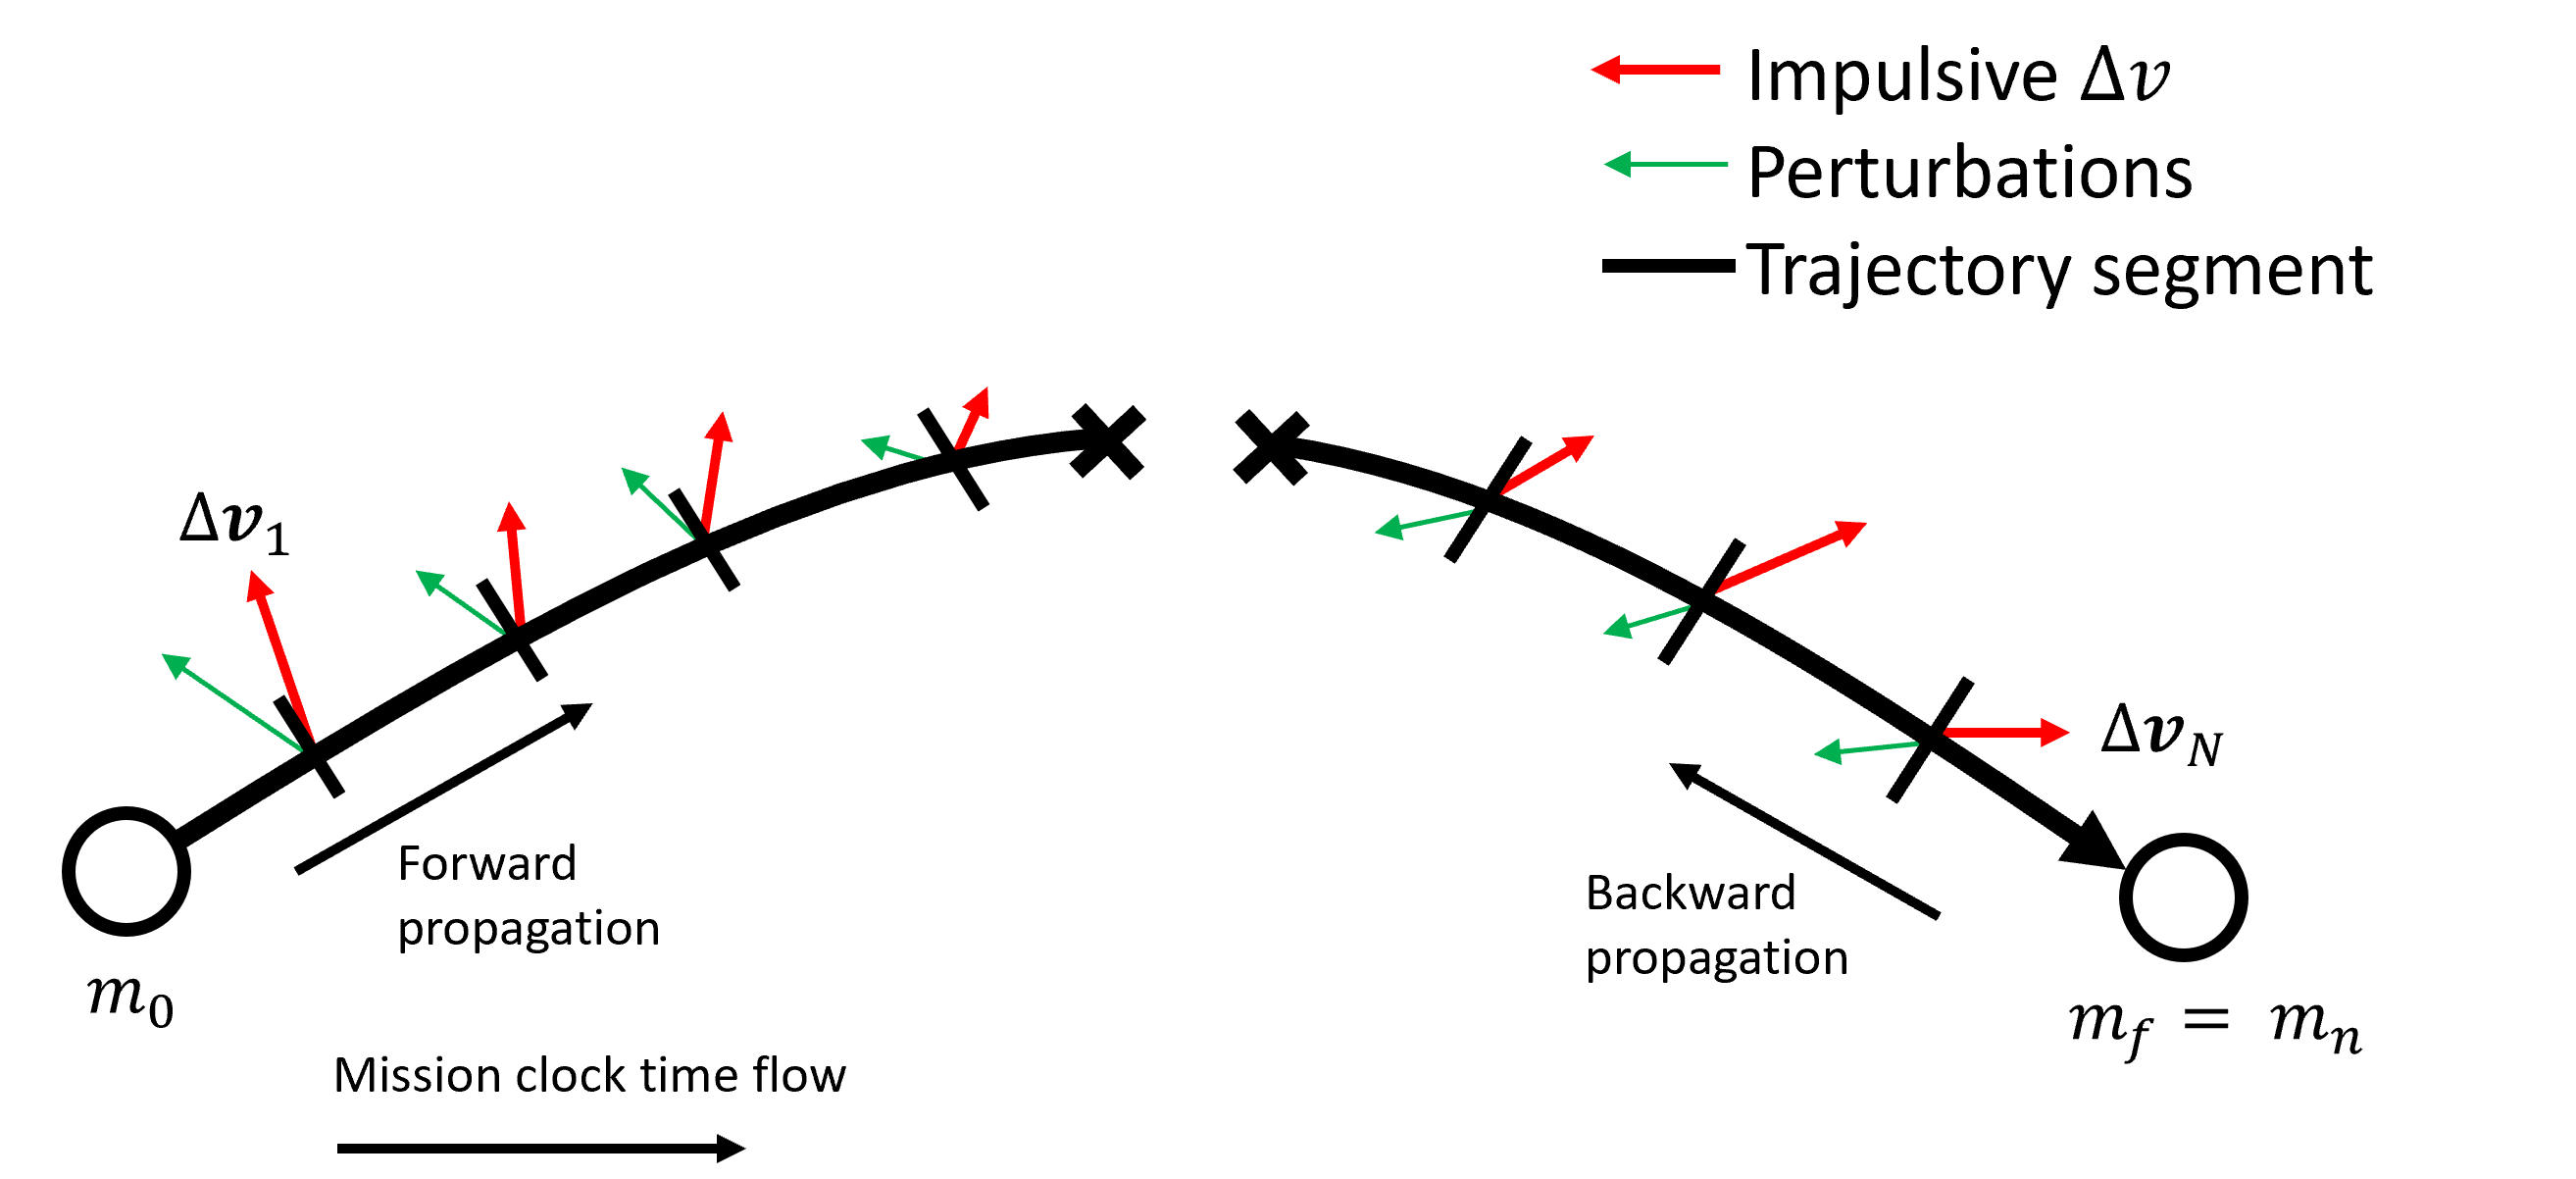
\includegraphics[width=0.9\textwidth]{../../shared_latex_inputs/images/mgalt.png}
        \caption{\acf{MGALT}}
    \end{figure}

\section{Finite Burn Low Thrust (FBLT)}
\label{sec:FBLT}

    \acf{FBLT} is identical to \ac{MGALT} except that numerical integration is used to propagate the equations of motion for the spacecraft rather than the Sims-Flanagan transcription. The central body, thrust, and perturbing forces (if used) sum to apply a net acceleration to the spacecraft, which is integrated with a Runge-Kutta method to generate the spacecraft trajectory. This gives a more realistic trajectory than \ac{MGALT}.

    \begin{figure}[H]
        \centering
        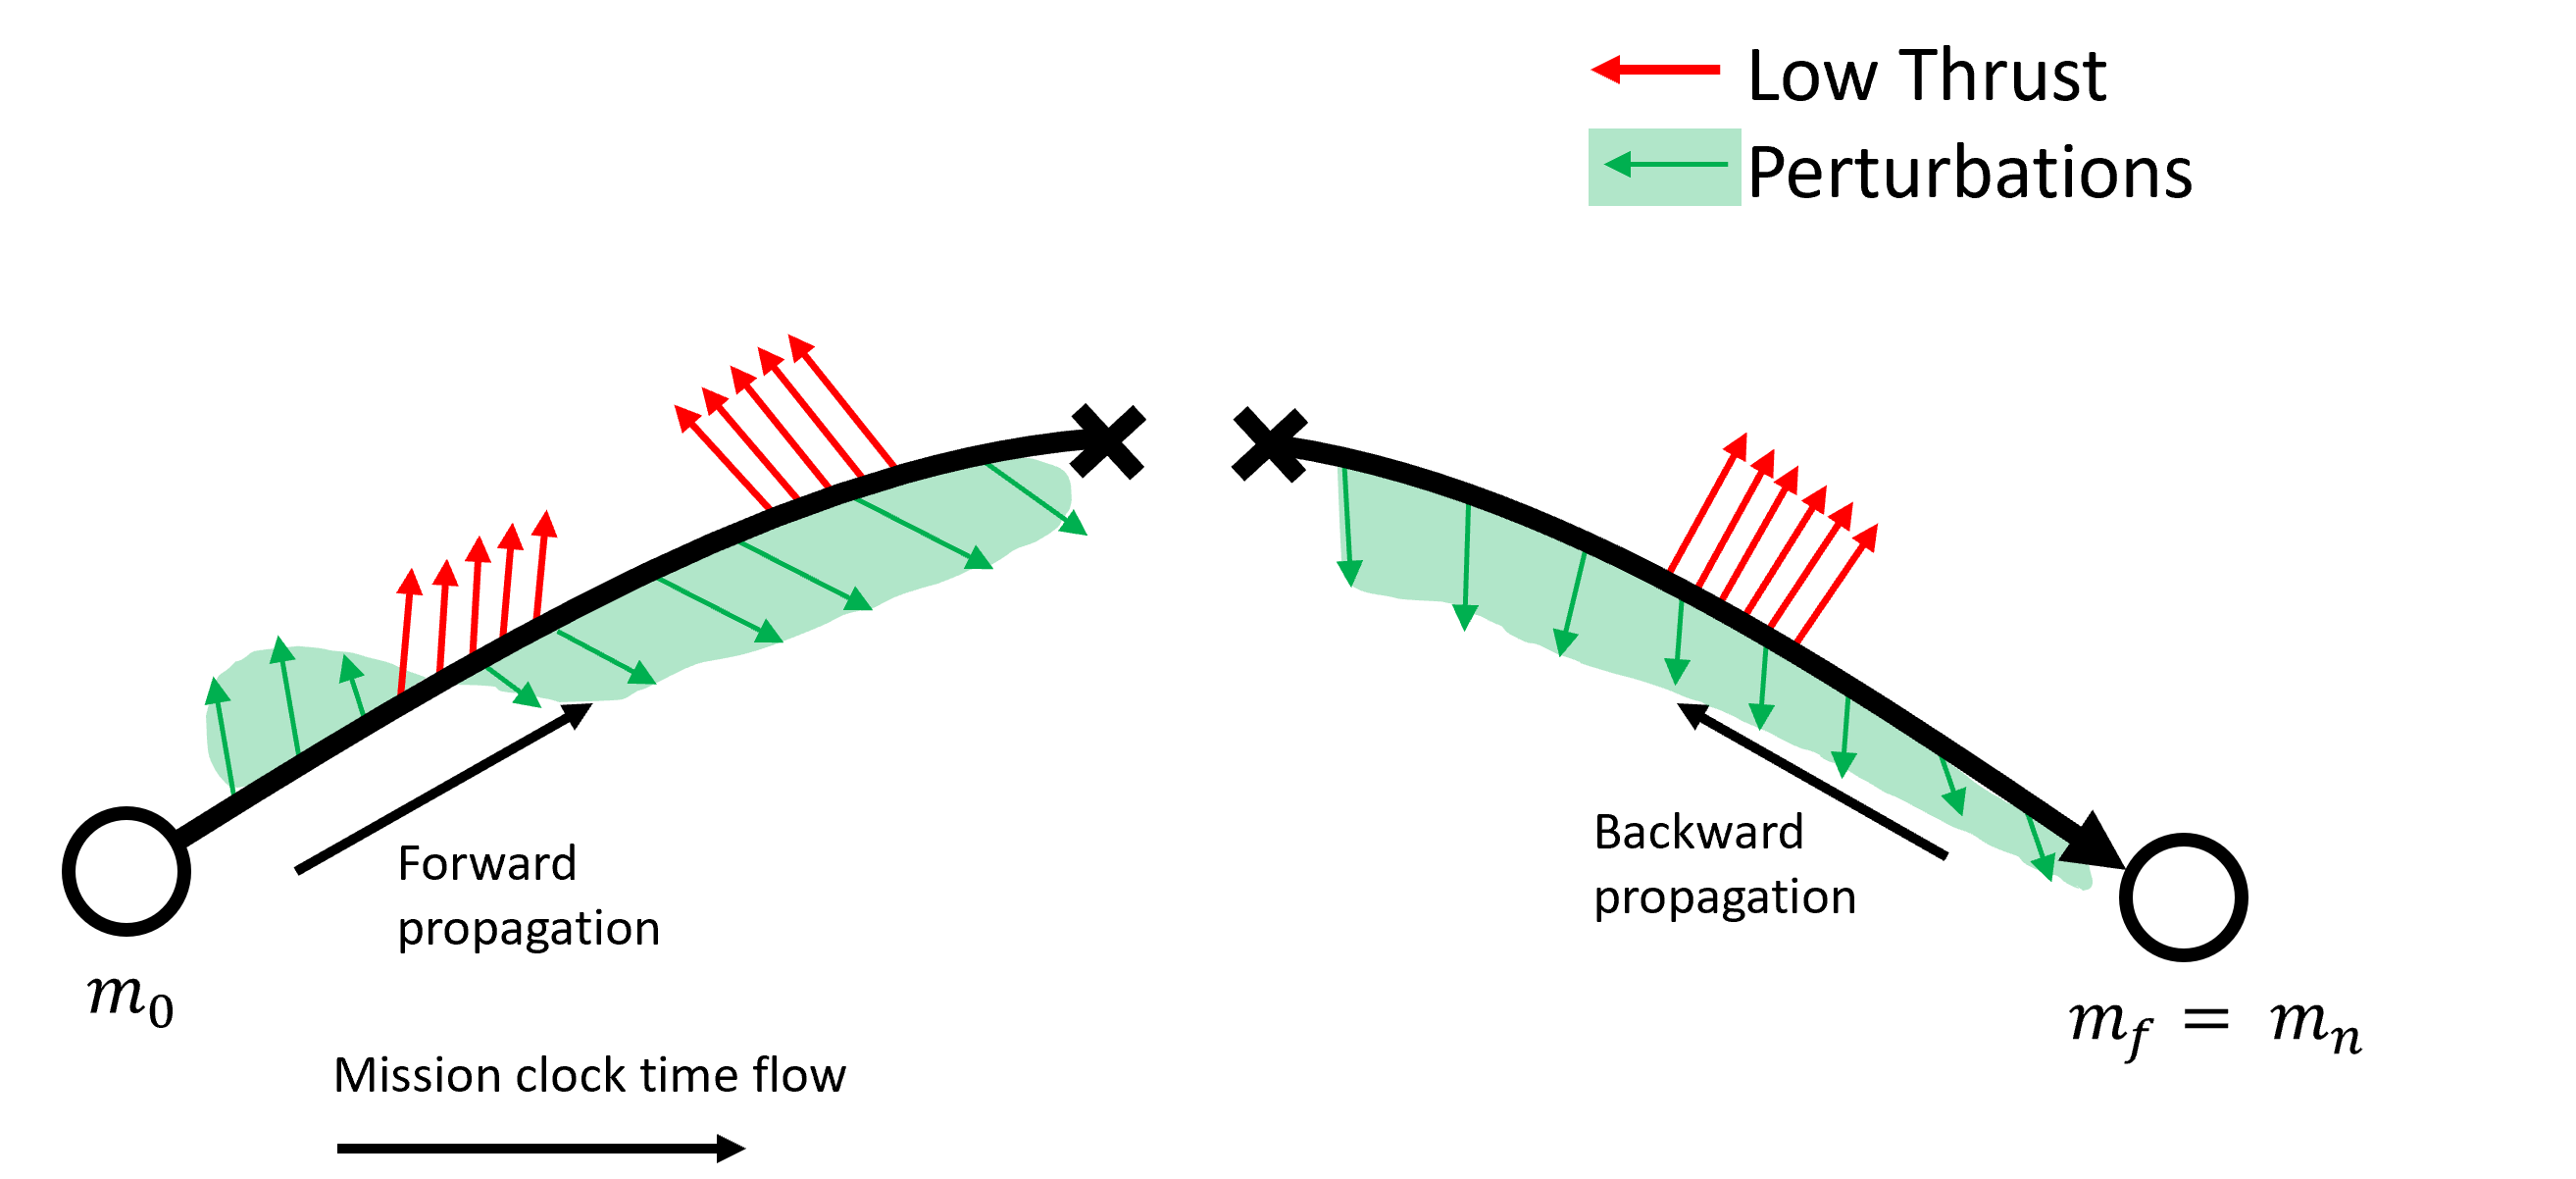
\includegraphics[width=0.9\textwidth]{../../shared_latex_inputs/images/fblt.png}
        \caption{\acf{FBLT}}
    \end{figure}

\section{Coast Phase}
\label{sec:coast_phase}

    Like the name implies, Coast Phase has no spacecraft thrust. It can be propagated with either Kepler (and no perturbing forces) or Integrator with optional perturbing forces. For a Coast Phase, the ``Integrator time step size'' set on the ``Physics Options'' tab is always overridden by the forward/backward half-phase step size values on the ``Journey Options'' tab. 


\section{Parallel Shooting Finite Burn (PSFB)}
\label{sec:parallel_shooting_finite_burn}
\ac{PSFB} is a phase transcription which models the path of a low-thrust spacecraft using direct parallel-shooting and a high-fidelity model of both the natural and spacecraft dynamics. \ac{PSFB} integrates the full set of dynamics with an explicit Runge-Kutta method with all central body, thrust, and perturbing forces (if used) applied. Since \ac{PSFB} is a parallel-shooting method and all steps propagate forward in time, each time-step encodes the left-hand state in the decision vector and includes a set of continuity constraints to enforce equivalency between the encoded left-hand state and the previous step's propagated right-hand state. This parallel-shooting method allows for easy implementation of maneuver constraints as compared to the two-point shooting used in \ac{FBLT}. 

\noindent The controls are piecewise constant across a segment. Users may choose to allow more than one control opportunities per segment when setting the Journey options. This option appears as ``Number of interior control points'' in the Journey Options tab. When more than one control opportunities are selected, the segment is broken into equal-length control steps. \ac{EMTG} has a high-fidelity duty cycle variant of \ac{PSFB} that is used when a realistic duty cycle option is selected. The duty cycle is discussed in more detail in Section \ref{sec:spacecraft_options}.

\begin{figure}[H]
    \centering
    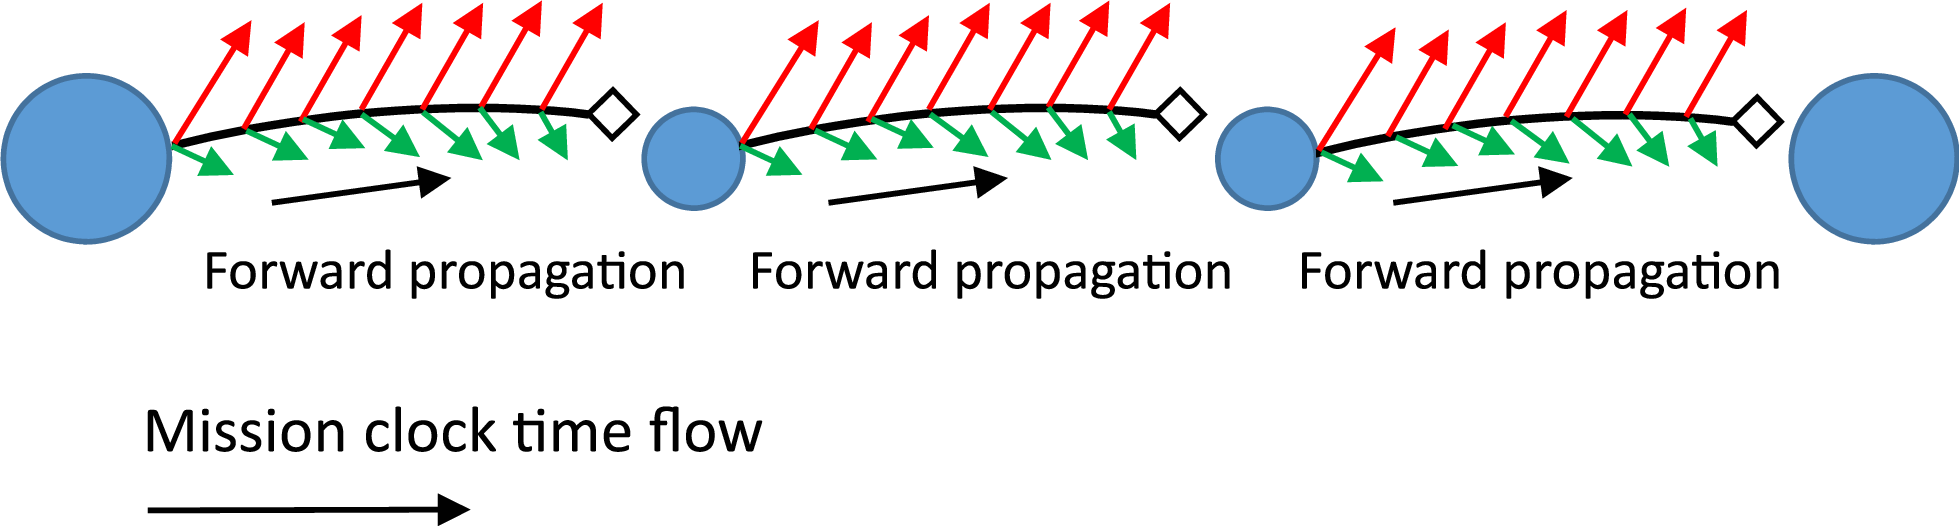
\includegraphics[width=0.9\textwidth]{../../shared_latex_inputs/images/PSFB_with_perturbations.png}
    \caption{\acf{PSFB}}
\end{figure}


\section{Parallel Shooting Bounded Impulse (PSBI)}
\label{sec:parallel_shooting_bounded_impulse}
\ac{PSBI} combines the Sims-Flanagan transcription with \ac{EMTG}'s base parallel-shooting phase classes, resulting in a low-fidelity parallel-shooting transcription. The low-thrust acceleration is modeled as a bounded impulse in the center of each time step, similar to the \ac{MGALT} transcription. Since \ac{PSBI} is a parallel-shooting method and all steps propagate forward in time, each time-step encodes the left-hand state in the decision vector and includes a set of continuity constraints to enforce equivalency between the encoded left-hand state and the previous step's propagated right-hand state. This parallel-shooting method allows for easy implementation of maneuver constraints as compared to the two-point shooting used in \ac{MGALT}. 

\begin{figure}[H]
    \centering
    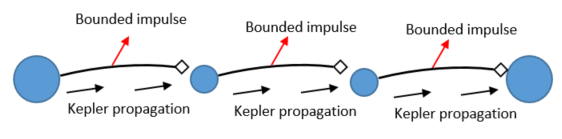
\includegraphics[width=0.9\textwidth]{../../shared_latex_inputs/images/PSBI.png}
    \caption{\acf{PSBI}}
\end{figure}



\section{Probe Entry Phase}
\label{sec:probe_entry}
Probe Entry Phase is a special phase type that tracks both the trajectory of the spacecraft and that of an entry probe which separates from the spacecraft. Following separation, the probe and spacecraft are propagated separately but for the same time of flight. The entry probe propagates to some point defining atmospheric entry and then to some surface target or parachute open state. The spacecraft performs a divert maneuver to enter some desired final state, defined by the Journey arrival conditions. 

\noindent This phase type derives from the \ac{MGAnDSMs} base class and thus inherits the same departure and arrival criteria for the main spacecraft. To handle the probe, an additional arrival event is introduced to define the desired target location for the probe independent of the rest of the problem. This right-hand boundary is modeled as a Free Point Intercept, thus when using the Probe Entry Phase mission type users must set some arrival elements using the same interface as any Free Point departure or arrival class. Separation is modeled using a user-defined constant separation impulse in Newton-seconds. This impulse is applied in the direction of the probe's velocity vector at entry.  

\noindent Since Probe Entry Phase inherits from \ac{MGAnDSMs}, this is done using a two-point shooting method with a set of match points linking the forward and backward half-phases. Since the probe does not perform maneuvers after separation, the match point location is specified as a fraction of the phase time of flight, which is a user-defined constant. This allows users to force the match point to be nearer to the right-hand boundary condition, allowing small time steps to be used when the probe is near the planet. This allows some representation of atmospheric entry. The second coast subphase following the match point then includes a unique time of flight decision variable to allow the optimizer to determine the arrival event.

\noindent Since the spacecraft is propagated alongside the probe, its propagation also inherits from \ac{MGAnDSMs} and thus uses the expected two-point shooting method. The match point for the propagation of the spacecraft is attached to the divert maneuver and may be placed in any permitted location in the phase just as maneuvers are in an \ac{MGAnDSMs} phase. Effectively, the spacecraft operates as if it is a normal \ac{MGAnDSMs} phase, with an initial mass loss equal to the weight of the entry probe.

\noindent An additional constraint is enforced on the distance between the probe and the spacecraft to ensure the solution maintains a reasonably high-bandwidth communication between the entry probe and the carrier spacecraft. This constraint is applied on the state at the end of the probe's trajectory and the state at the end of the spacecraft's trajectory and is set by the user in the Journey Options via the ``Probe communication distance bounds (km)'' input.


\begin{figure}[H]
    \centering
    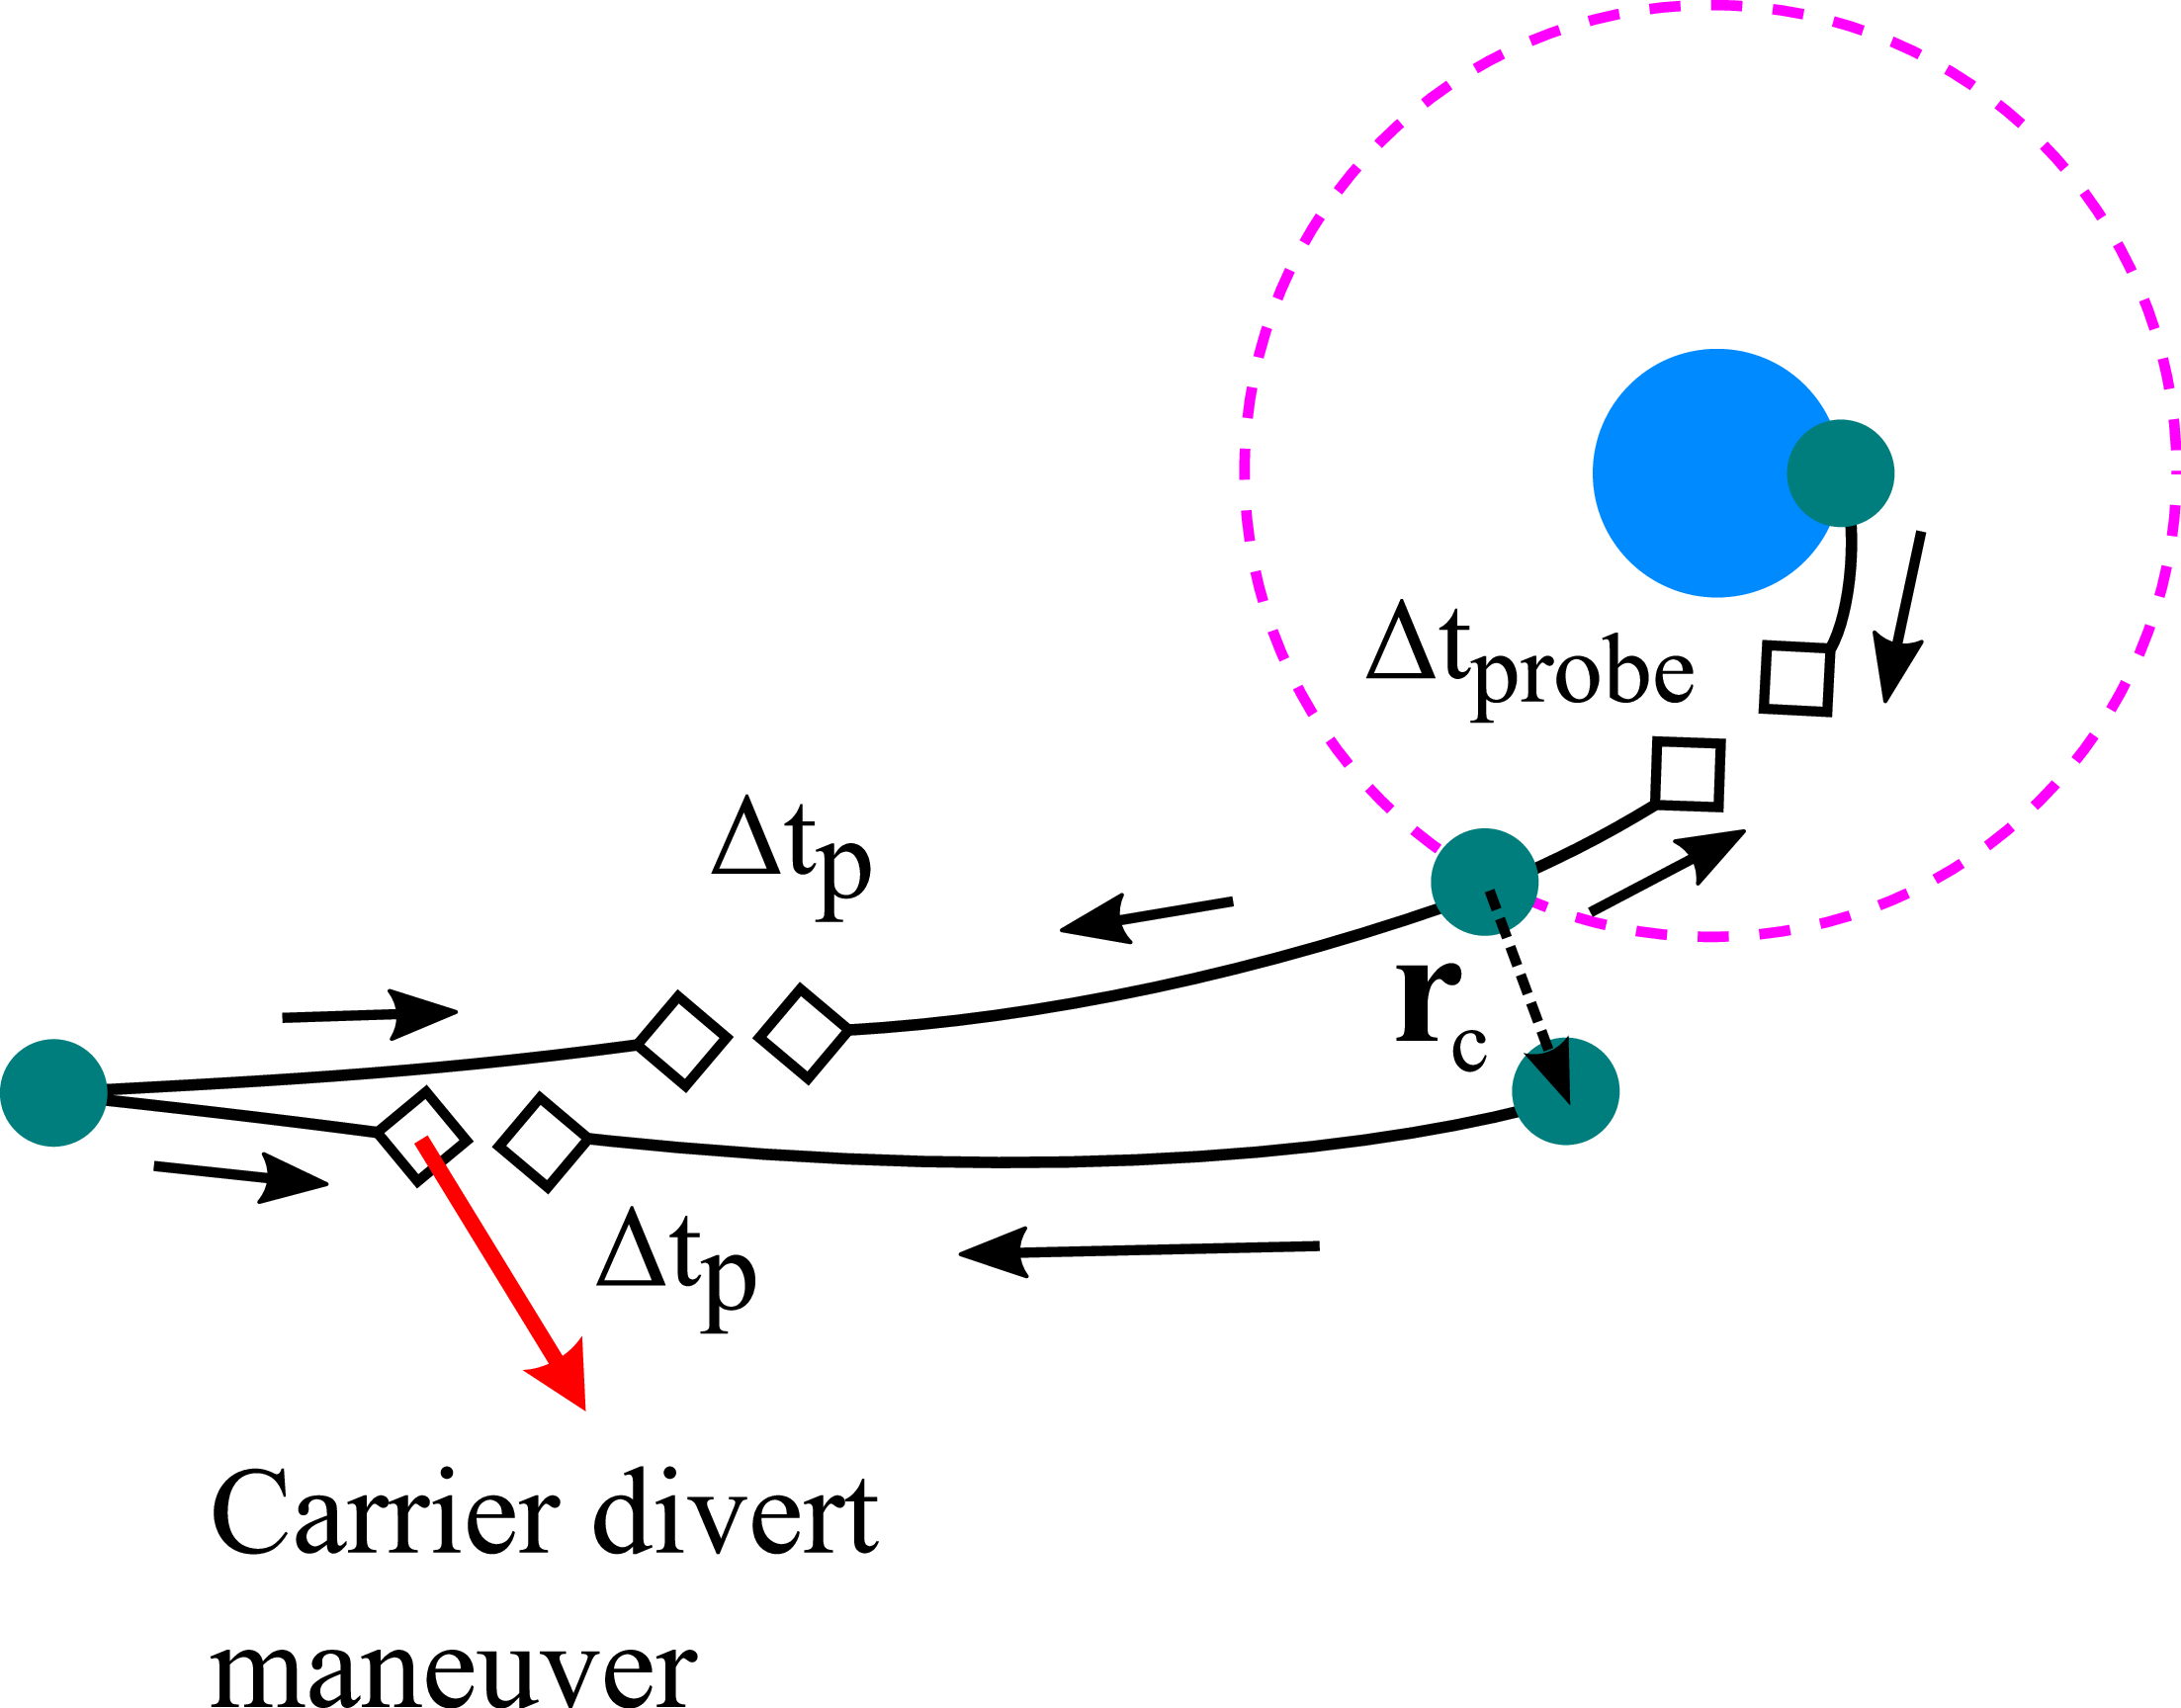
\includegraphics[width=0.9\textwidth]{../../shared_latex_inputs/images/ProbeEntryPhase_zoom.png}
    \caption{Probe Entry Phase}
\end{figure}



